\documentclass[../main.tex]{subfiles}
\begin{document}

% E' consentito agli studenti che ne facciano richiesta al proprio relatore, di formulare la tesi in lingua inglese e in ogni altra lingua straniera di uno stato dell’Unione Europea, purché il testo venga preceduto da un'ampia sintesi (dell'ordine di 10 pagine) dei contenuti in lingua italiana. All'atto della presentazione dei prescritti moduli in Segreteria studenti, il titolo della tesi dovrà essere definito sia in lingua italiana sia nella lingua straniera ed entrambe le formulazioni dovranno essere riportate sull'intestazione della tesi stessa.
\section{Sintesi italiana - Abstract}
Lo sviluppo software in ambito Automotive é un campo in continua espansione.La logica di controllo presente in centralina controlla tutti gli aspetti del veicolo, dalla temperatura nell'abitacolo, alla velocità su strada fino ai sistemi di guida autonoma \gls{ADAS}. 
Le linee di codice presenti nei veicoli sono passate da quasi zero a qualche milione in un arco temporale di circa 50 anni. La crescita nella complessità ha richiesto una grande espansione nel campo dello sviluppo software per applicazioni autoveicolo. La complessità dietro i processi traspare nella prima parte della tesi, dove vengono analizzati i processi di sviluppo software all'interno del mondo Automotive, seguendo le metodologie usate presso \gls{BMW}.\\
Il focus si sposta poi sull'argomento principale della tesi, ovvero lo sviluppo di una pipeline dati per l'analisi di informazioni relative alle versioni di software per la centralina. Durante il ciclo di sviluppo software nella centralina una grande quantità di dati viene generata. Molto spesso questi dati vengono usati solamente dai dipartimenti responsabili dello sviluppo di una certa funzionalità e a volte, solamente dal singolo sviluppatore. Manca un sistema centralizzato che fornisca una visione d'insieme su tutto il processo.\\
Partendo da questa richiesta la tesi riporta il processo di sviluppo di un infrastruttura che possa attivamente salvare informazioni in un database e fornire un feedback agli sviluppatori tramite una visualizzazione grafica dei dati (Dashboard). Lo scopo del progetto é proprio questo, ovvero creare una Dashboard che possa fornire in tempo reale informazioni sullo stato di avanzamento dello sviluppo del software.\\
Il lavoro riportato nella tesi, parte con la creazione dei processi che portano alla generazione dei dati. Dopodiché lo sviluppo continua con la descrizione della creazione dell'infrastruttura che possa supportare il flusso di dati dalla parte di generazione fino alla Dashboard. 

\section{Sintesi italiana - Introduzione}
Nel capitolo di introduzione viene trattato il tema del sistema automobile. Partendo da una semplificazione del modello automobile, riportato come semplice sistema ad anello chiuso la trattazione si sviluppa fino a definire la più complessa dicotomia elettronica meccanica nel veicolo, come riportato in Figura \ref{fig:schemaablocchi}.
\begin{figure}[ht]
        \begin{center}
  \begin{tikzpicture}[auto, node distance=3cm,>=latex', scale=0.7,transform shape]
            \node [input1, name=input] {};
            \node [sum1, right=of input] (sum) {};
            \node [sum, right=of sum] (sum_A) {};
            \node [block, right=of sum_A] (controller) {$Electronics$};
            \node [block, right=of controller] (mechanics) {$Mechanics$};
            \node [output1, right=of mechanics] (output) {};
            \draw [draw,->] (input) -- node {$User\; inputs$} (sum);
            \draw [->] (sum) -- node {} (sum_A);
            \draw [->] (sum_A) -- node {} (controller);
            \draw [->] (controller) -- node {} (mechanics);
            \draw [->] (mechanics) -- node [name=y] {$(speed,\; position..)$}(output);
            \draw [->] (mechanics) -- ++ (0,-2) -| node [pos=0.99] {$-$} (sum_A);
            \draw [->] (y) -- ++ (0,-4) -| node [pos=0.99] {$-$} (sum);
            % \node [container,fit=(controller) (mechanics) (sum_A)] (container) {};
            \end{tikzpicture}
        \end{center}
        \caption{Schema a blocchi di un'automobile}
        \label{fig:schemaablocchi}
    \end{figure}
La trattazione continua trattando il tema del software per centraline. In generale il software per \gls{ECU} può essere paragonato a software per sistemi embedded di tipo Real Time, ovvero dove la correttezza della risposta dipende non solo da una correttezza sul piano logico ma anche sul piano temporale. Con questo vengono di seguito introdotte le problematiche tipiche di sistemi real time, in modo da creare un'idea della complessità delle informazioni presenti nel software. 
Nella parte finale del capitolo viene poi introdotto il concetto di compilatore, il quale ha la funzione di ricevere come input il codice, sviluppato in Matlab che definisce il funzionamento della centralina e generare come output il codice compilato che potrà poi essere letto dall'organo centralina stesso.//
Il problema trattato nella tesi si lega a questo argomento. Infatti durante il processo di compilazione codice, il quale in \gls{BMW} è fatto da un compilatore sviluppato internamente, si ha la generazione di una grande mole di dati riguardanti lo stato del processo. In generale differenti dipartimenti e differenti persone si occupano di singoli parti di questo processo. I dati non sono quindi solamente rilevanti in termine di mole ma sono anche divisi su differenti persone, rendendo complesso avere una visione d'insieme sullo stato del processo. A questo proposito l'obiettivo della tesi è quello di sviluppare una struttura che possa salvare i dati, processarli e fornirli a tutti gli utenti tramite una visualizzazione grafica. L'obiettivo di questo progetto è quello di migliorare il feedback per i singoli sviluppatori e fornire una visione d'insieme ad ora mancante. 
\section{Sintesi italiana - Agile e Scrum}
Il capitolo introduce e sviluppa concetti legati alle modalità di lavoro utilizzate nel campo dello sviluppo software. Inizialmente viene trattato il concetto di filosofia Agile, partendo da una breve introduzione storica fino alla prima teorizzazione, con i relativi punti salienti del Manifesto della filosofia Agile \cite{beck2001agile}. La trattazione dei modelli di lavoro Agile continua trattando alcune applicazioni reali della suddetta filosofia come lo Scrum (Figura \ref{fig:agilesrre}).\\
Lo Scrum fornisce una struttura utile ad applicare modelli di lavoro Agile. La struttura si compone di vari parti, quali:
\begin{itemize}
    \item Scrum team, gruppo di persone con una gerarchia definita e all'interno del quale ogni persona ha un ruolo definito, legato allo Scrum.
    \item Eventi, il ciclo di sviluppo prodotto è basato su una serie di eventi, che insieme definiscono il cosiddetto Scrum Sprint.
    \item Regole, le quali uniscono e regolano non solo l'interazione tra ruoli ma definiscono anche ciò che accade nei singoli eventi e gli artefatti necessari per controllare l'intero processo.
    \item Artefatti, serie di strumenti utili a tracciare il processo di sviluppo.
\end{itemize}
Gli aspetti principali dello sviluppo prodotto secondo metodologie Scrum sono legati al continuo feedback all'interno del ciclo di lavoro, in modo da avere un costante miglioramento dell'output. Inoltre una ulteriore differenza con le metodologie  classiche si ritrova nella continua accettazione, durante tutto il ciclo di progettazione di nuove specifiche per il prodotto, aspetto molto importante in progetti in continua evoluzione.\\
Il capitolo tratta dunque in modo completo tutto ciò che riguarda la metodologia di lavoro Scrum, e la sua applicazione nel campo dello sviluppo software. In conclusione viene presentato un esempio di come un prodotto può essere sviluppato in modalità Scrum, facendo un paragone diretto con le metodologie classiche in modo tale da evidenziare le differenze e i punti di forza di entrambe.
\begin{figure}
    \centering
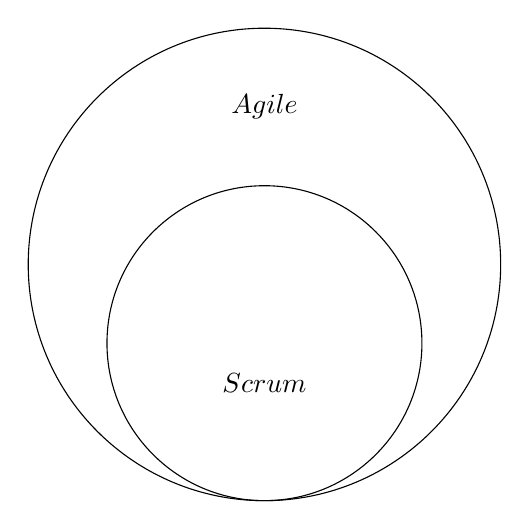
\begin{tikzpicture}
\draw[] (4.5,2) circle[radius = 3];
\node [at={(4.5,4)}] {$Agile$};
\draw [] (4.5,1) circle [radius =2];
\node [at = {(4.5,0.5)}] {$Scrum$};
\end{tikzpicture} 
    \caption{Relazione Agile - Scrum}
    \label{fig:agilesrre}
\end{figure}
% Sintesi ECU strucutre
\section{Sintesi italiana - Struttura ECU}
Nel capitolo viene fornita un'introduzione iniziale alle centraline presenti nei veicoli. Le centraline possono infatti essere pensate come complesse versioni di sistemi embedded.\\
Dopo aver introdotto le principali centraline presenti nel veicolo il capitolo continua nella trattazione descrivendo l'organizzazione delle \gls{ECU} dal punto di vista dell'hardware e del software. Il focus si sviluppa sulla parte software, in quanto quella che più importante per l'obiettivo della tesi.\\
Nella parte legata al software seguendo una logica top down, si parte infatti dallo sviluppo delle logiche di controllo passando per l'interfaccia usata tra hardware e software fino ad arrivare a metodologie di comunicazione utilizzate sull'hardware delle centraline. Il capitolo inizia con l'introduzione del Model Based Design  e i relativi metodi di astrazione utile a sviluppare modelli di sistemi complessi e in particolare a sviluppare logiche di controllo per i suddetti modelli. Un esempio di sviluppo in Model Based Design viene riportato. Il capitolo continua introducendo lo standard \gls{AUTOSAR}, architettura create per interfacciare hardware e software in sistemi real time in campo Automotive come le \gls{ECU}. Lo standard \gls{AUTOSAR} introduce uno strato di astrazione (Figura \ref{fig:autosar}) tra il codice embedded e l'hardware della centraline, permettendo una maggior facilità nello sviluppo ma sopratutto una più elevata portabilità del codice su differenti versioni e tipologie di centraline. Questo aspetto è di vitale importanza sopratutto per l'incremento che lo sviluppo software sta avendo, richiedendo molte più risorse sopratutto dal punti di vista economico.
\begin{figure}[h]
    \centering
    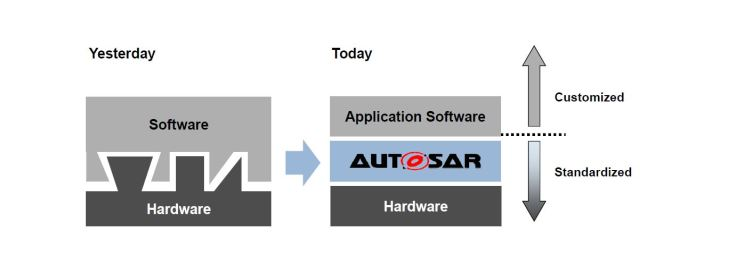
\includegraphics[width=\linewidth]{images_folder/autosarcapture.jpg}
    \caption{Standard AUTOSAR}
    \label{fig:autosar}
\end{figure}

\section{Sintesi italiana - Software build e integrazione continua}
Il capitolo tratta temi legati ai concetti di Software Configuration Managment. Questi concetti definiscono le basi di come sviluppare software. E' importante evidenziare il fatto che a differenza delle metodologie di sviluppo prodotto, le quali definiscono linee guida su come sviluppare un generico prodotto, i concetti di \gls{SCM} definiscono come sviluppare software. L'unione dei due è il metodo utilizzato per sviluppare software in \gls{BMW}, seguita dunque anche per lo sviluppo del progetto trattato nella tesi.\\
Dopo un'introduzione legata ai concetto di \gls{SCM} il capitolo si sviluppa definendo il concetto di Software build. L'artefatto sul quale il progetto si basa è infatti un Build software responsabile dello sviluppo di codice compilabile per la centralina. In Figura \ref{fig:approachbuildingsoftware} viene riportato uno schema sul quale lo sviluppo di tale software è basato.
\begin{figure}[H]
    \begin{center}
        \begin{tikzpicture}[scale=0.7,transform shape,node distance=1cm and 1cm,>=latex']
        \node [input3, left =of sum ] (requirements) {$Requirements$};
        \node [sum2, right =of requirements] (sum) {};
        \draw [->] (requirements) -- node [left] {} (sum);
        \node [block, right= of sum] (changes) {$Changes\;Implementation$};
        \draw [->] (sum) -- node {} (changes);
        \node [block, right =of changes] (build) {$Build$};
        \draw [->] (changes) -- node {} (build);
        \node [block, right =of build] (test) {$Test$};
        \draw [->] (build) -- node {} (test);
        \node [block, right =of test] (review) {$Review$};
        \draw [->] (test) -- node {} (review);
        \draw[->] (review)--++(-90:1) coordinate (A)--++(-90:2.5) coordinate (B)-|(sum);
        \node [block, above =of review] (versioning) {$Versioning$};
        \draw [->] (review) -- node [above, pos=0.79] {} (versioning);
        \node [block, above =of versioning] (repository) {$Repository$};
        \draw [->] (versioning) -- node {} (repository);
        
        \node [block, above =of sum] (branch) {$Branch$};
        \draw [<-] (sum) -- node {} (branch);
        \node [block, above =of branch] (Baseline) {$Baseline$};
        \draw [<-] (branch) -- node {} (Baseline);
        \node [sum2, above =of Baseline] (sum1) {};
        \draw [<-] (Baseline) -- node {} (sum1);
        \draw [->] (repository) |- node {} (sum1);
        
        \node [input2, name=input, left =of sum1] {};
        \draw [draw,->] (input) -- node [above left] {$Other\;changes$} (sum1);
        
        \end{tikzpicture}
    \end{center}
    \caption{Approccio al modello di Build}
    \label{fig:approachbuildingsoftware}
\end{figure}
Nella parte finale del capitolo il suddetto Build software, il cui nominativo è EA-build viene introdotto  e alcuni dei concetti utilizzati vengono analizzati. Il focus del capitolo è però anche quello dell'integrazione continua, concetto innovativo legato alla produzione di artefatti. 
\section{Sintesi italiana - Database}
All'interno del processo di analisi dei data provenienti dalle versioni software per le centraline un ruolo fondamentale è rivestito dal database relazionale di tipo \gls{SQL}. Nel capitolo vengono introdotti i concetti legati allo sviluppo di un database.\\
Nella parte introduttiva viene analizzata la convenienza dell'utilizzo di un database di tipo relazionale rispetto ad altri modelli di salvataggio dati. \\
Dopo aver introdotto i concetti principali legati ai database e ai sistemi che ne arbitrano il funzionamento viene introdotto il meccanismo tramite il quale il database viene collegato al Software di build (Figura \ref{fig:tcpdbita}). Dal momento che il software di build è scritto in linguaggio Python viene scelta una libraria per la connessione.\\
Nel capitolo infine è spiegato come avviene il collegamento tramite un semplice esempio di implementazione. 


\tikzset{every picture/.style={line width=0.75pt}} %set default line width to 0.75pt        
\begin{figure}
    \centering
\begin{tikzpicture}[x=0.75pt,y=0.75pt,yscale=-0.8,xscale=0.8]
%uncomment if require: \path (0,300); %set diagram left start at 0, and has height of 300

%Image [id:dp6531549605845597] 
\draw (386,154.71) node  {
\includegraphics[width=81pt,height=97.93pt]{images_folder/database.png}};
%Image [id:dp05605943116066481] 
\draw (216,156) node  {
\includegraphics[width=52.5pt,height=52.5pt]{images_folder/firewall-protection-2039809-1721228.png}};
%Image [id:dp383039570021823] 
\draw (64,102.71) node  {
\includegraphics[width=34.5pt,height=35.57pt]{images_folder/pc.png}};
%Image [id:dp5074894649578912] 
\draw (64,163.71) node  {
\includegraphics[width=34.5pt,height=35.57pt]{images_folder/pc.png}};
%Image [id:dp8452106454068984] 
\draw (63,223.71) node  {
\includegraphics[width=34.5pt,height=35.57pt]{images_folder/pc.png}};
%Image [id:dp3665068119749033] 
\draw (595.5,100.21) node  {
\includegraphics[width=48.75pt,height=51.32pt]{images_folder/935839-200.png}};
%Image [id:dp45105133171160383] 
\draw (595.5,160.21) node  {
\includegraphics[width=48.75pt,height=51.32pt]{images_folder/935839-200.png}};
%Image [id:dp1763171670611261] 
\draw (595.5,221.21) node  {
\includegraphics[width=48.75pt,height=51.32pt]{images_folder/935839-200.png}};
%Straight Lines [id:da21693223941443396] 
\draw    (100,101) -- (168.25,139.17) ;
\draw [shift={(170,140.14)}, rotate = 209.21] [color={rgb, 255:red, 0; green, 0; blue, 0 }  ][line width=0.75]    (10.93,-3.29) .. controls (6.95,-1.4) and (3.31,-0.3) .. (0,0) .. controls (3.31,0.3) and (6.95,1.4) .. (10.93,3.29)   ;
%Straight Lines [id:da3176124570414163] 
\draw    (99,220) -- (168.26,181.12) ;
\draw [shift={(170,180.14)}, rotate = 510.69] [color={rgb, 255:red, 0; green, 0; blue, 0 }  ][line width=0.75]    (10.93,-3.29) .. controls (6.95,-1.4) and (3.31,-0.3) .. (0,0) .. controls (3.31,0.3) and (6.95,1.4) .. (10.93,3.29)   ;
%Straight Lines [id:da8563188339305701] 
\draw    (100,159.14) -- (168,160.11) ;
\draw [shift={(170,160.14)}, rotate = 180.82] [color={rgb, 255:red, 0; green, 0; blue, 0 }  ][line width=0.75]    (10.93,-3.29) .. controls (6.95,-1.4) and (3.31,-0.3) .. (0,0) .. controls (3.31,0.3) and (6.95,1.4) .. (10.93,3.29)   ;
%Straight Lines [id:da10650658101917698] 
\draw    (260,160.14) -- (328,161.11) ;
\draw [shift={(330,161.14)}, rotate = 180.82] [color={rgb, 255:red, 0; green, 0; blue, 0 }  ][line width=0.75]    (10.93,-3.29) .. controls (6.95,-1.4) and (3.31,-0.3) .. (0,0) .. controls (3.31,0.3) and (6.95,1.4) .. (10.93,3.29)   ;
%Straight Lines [id:da8525254743123636] 
\draw    (439,120.14) -- (477.19,102) ;
\draw [shift={(479,101.14)}, rotate = 514.5899999999999] [color={rgb, 255:red, 0; green, 0; blue, 0 }  ][line width=0.75]    (10.93,-3.29) .. controls (6.95,-1.4) and (3.31,-0.3) .. (0,0) .. controls (3.31,0.3) and (6.95,1.4) .. (10.93,3.29)   ;
%Straight Lines [id:da9180864032323492] 
\draw    (440,200.14) -- (478.19,218.28) ;
\draw [shift={(480,219.14)}, rotate = 205.41] [color={rgb, 255:red, 0; green, 0; blue, 0 }  ][line width=0.75]    (10.93,-3.29) .. controls (6.95,-1.4) and (3.31,-0.3) .. (0,0) .. controls (3.31,0.3) and (6.95,1.4) .. (10.93,3.29)   ;
%Straight Lines [id:da15194220294106842] 
\draw    (440,161.14) -- (478,161.14) ;
\draw [shift={(480,161.14)}, rotate = 180] [color={rgb, 255:red, 0; green, 0; blue, 0 }  ][line width=0.75]    (10.93,-3.29) .. controls (6.95,-1.4) and (3.31,-0.3) .. (0,0) .. controls (3.31,0.3) and (6.95,1.4) .. (10.93,3.29)   ;
%Straight Lines [id:da09311856378325101] 
\draw    (521,101.14) -- (559,101.14) ;
\draw [shift={(561,101.14)}, rotate = 180] [color={rgb, 255:red, 0; green, 0; blue, 0 }  ][line width=0.75]    (10.93,-3.29) .. controls (6.95,-1.4) and (3.31,-0.3) .. (0,0) .. controls (3.31,0.3) and (6.95,1.4) .. (10.93,3.29)   ;
%Straight Lines [id:da43474826611768935] 
\draw    (521,160.14) -- (559,160.14) ;
\draw [shift={(561,160.14)}, rotate = 180] [color={rgb, 255:red, 0; green, 0; blue, 0 }  ][line width=0.75]    (10.93,-3.29) .. controls (6.95,-1.4) and (3.31,-0.3) .. (0,0) .. controls (3.31,0.3) and (6.95,1.4) .. (10.93,3.29)   ;
%Straight Lines [id:da13431673428420954] 
\draw    (521,221.14) -- (559,221.14) ;
\draw [shift={(561,221.14)}, rotate = 180] [color={rgb, 255:red, 0; green, 0; blue, 0 }  ][line width=0.75]    (10.93,-3.29) .. controls (6.95,-1.4) and (3.31,-0.3) .. (0,0) .. controls (3.31,0.3) and (6.95,1.4) .. (10.93,3.29)   ;
%Image [id:dp9305152591758974] 
\draw (501.14,216.55) node  {
\includegraphics[width=24.22pt,height=26.17pt]{images_folder/lock.png}};
%Image [id:dp22011543040409642] 
\draw (501.14,156.55) node  {
\includegraphics[width=24.22pt,height=26.17pt]{images_folder/lock.png}};
%Image [id:dp43535330126349736] 
\draw (501.14,96.55) node  {
\includegraphics[width=24.22pt,height=26.17pt]{images_folder/lock.png}};

\end{tikzpicture}
    \caption{Schema di connessione al database}
    \label{fig:tcpdbita}
\end{figure}
\section{Sintesi italiana - Sviluppo della Dashboard}
Il capitolo legato allo sviluppo della Dashboard è il capitolo principale e quello che riprende i concetti trattati precedentemente  e li lega allo sviluppo della Dashboard stessa.\\
Il processo di sviluppo software prevede infatti la generazione di un'elevata mole di dati, i quali sono utilizzati dai singoli sviluppatori per avere un feedback sul processo di sviluppo software. Questi dati sono attualmente salvati sotto varie forme e in differente piattaforme. Manca una struttura generale che possa salvare e fornire una visualizzazione dei dati all'interno di una singola piattaforma. La Dashboard, come punto finale, e la struttura che c'è dietro a questa vuole fornire un modo per avere una visione d'insieme centralizzata sul processo, disponibile a tutti gli sviluppatori.\\
Come sottolineato, la Dashboard e dunque la visualizzazione grafica dei dati è solamente il gradino finale di un processo che si articola in più punti, di seguito riportati:
\begin{itemize}
    \item Sorgente dei dati, i dati che vengono generati nel processo di compilazione software devono essere raccolti e inviati al database. Nel capitolo viene descritta la modalità con la quale questa integrazione è stata fatta. Inoltre vengono trattate alcune idee utilizzate per rendere efficiente questo scambio di dati.
    \item Salvataggio dei dati, il salvataggio dei dati avviene in un database di tipo \gls{SQL} relazionale. Qui i dati vengono salvati sotto forma di tabelle collegate tra di loro per sfruttare al meglio le potenzialità dei database relazionali e ottimizzare lo spazio richiesto.
    \item Visualizzazione grafica dei dati, questo passaggio è quello dove la Dashborad viene creata. La sezione relativa tratta come tramite una rielaborazione dei dati via linguaggio SQL dal database venga creata una visualizzazione interattiva dei dati tramite grafici, \gls{KPI} e tabelle.
\end{itemize}
In Figura \ref{fig:pipelineita} viene riportato uno schema riassuntivo sulla struttura della pipeline dati, termine che vuole sottolineare come i dati viaggino dal software che li genera fino alla Dashborad dove possono essere idealmente istantaneamente visibili all'utente finale, in questo caso gli sviluppatori.
\begin{figure}[h]
    \centering
    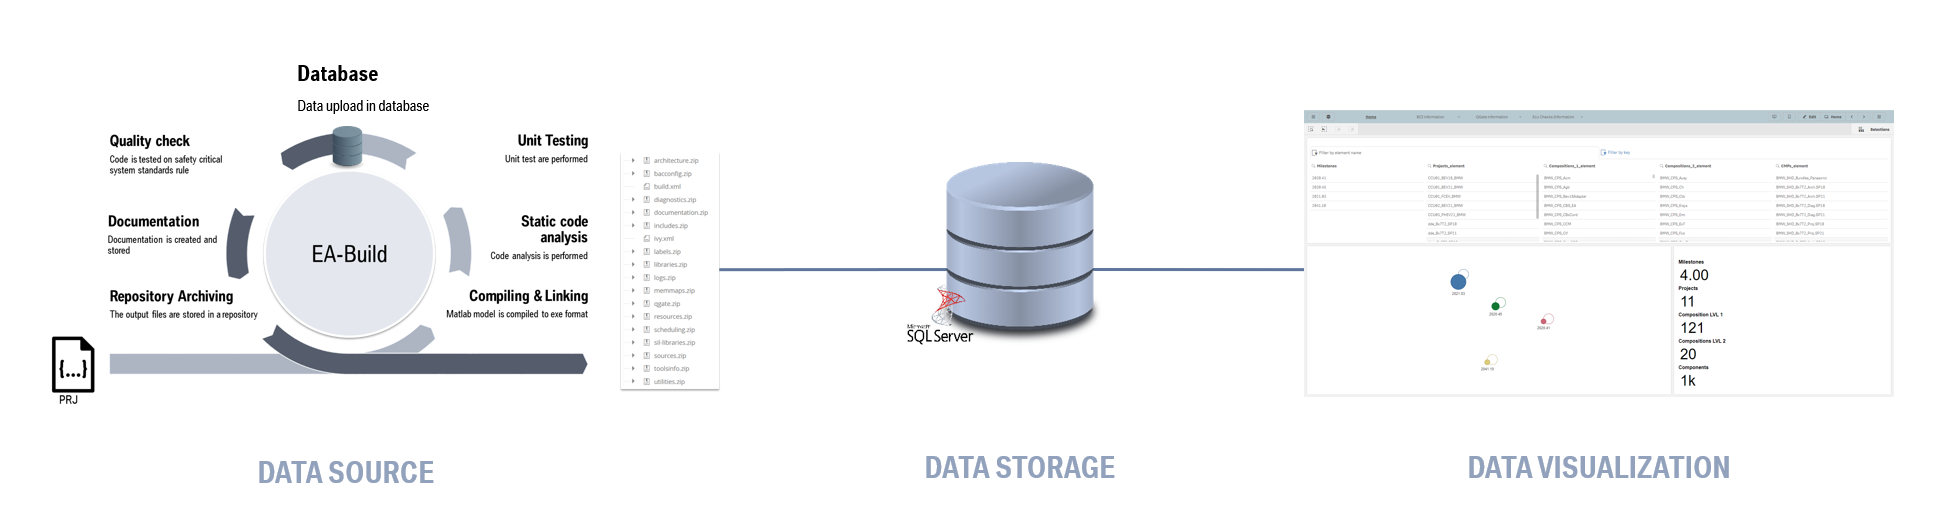
\includegraphics[width=\linewidth]{images_folder/pipeline_1.png}
    \caption{Struttura della pipeline dati}
    \label{fig:pipelineita}
\end{figure}
\section{Sintesi italiana - Conclusioni}
Le conclusioni analizzano i risultati e riflettono sugli obiettivi prefissati per la tesi nel capitolo introduttivo. 
L'analisi fatta del processo di sviluppo software, visto dal punto di vista interno in una grande azienda come \gls{BMW}. La complessità dei processi viene trattata durante tutta la prima parte della tesi, definendo passo per passo i vari processi e quindi affrontando la complessità dell'insieme pezzo per pezzo.\\
In secondo luogo lo sviluppo della Dashboard, la quale fornisce uno strumento utile per rendere ancora più efficacie il feedback sullo stato del processo. Nelle conclusioni vengono trattati i punti di forza e di debolezza dell'attuale implementazione e lo stato finale del progetto.
\cleardoublepage
\end{document}